\chapter{Interfaz de usuario}
\section{Diseño}
{\color{red} Explicar por qué es necesaria}

En primer lugar, hice un diseño aproximado para la interfaz de usuario que
necesitaba haciendo uso de \textbf{\textit{QT Design Studio}}. Obteniendo el
siguiente resultado:

\begin{figure}[h]
    \centering
    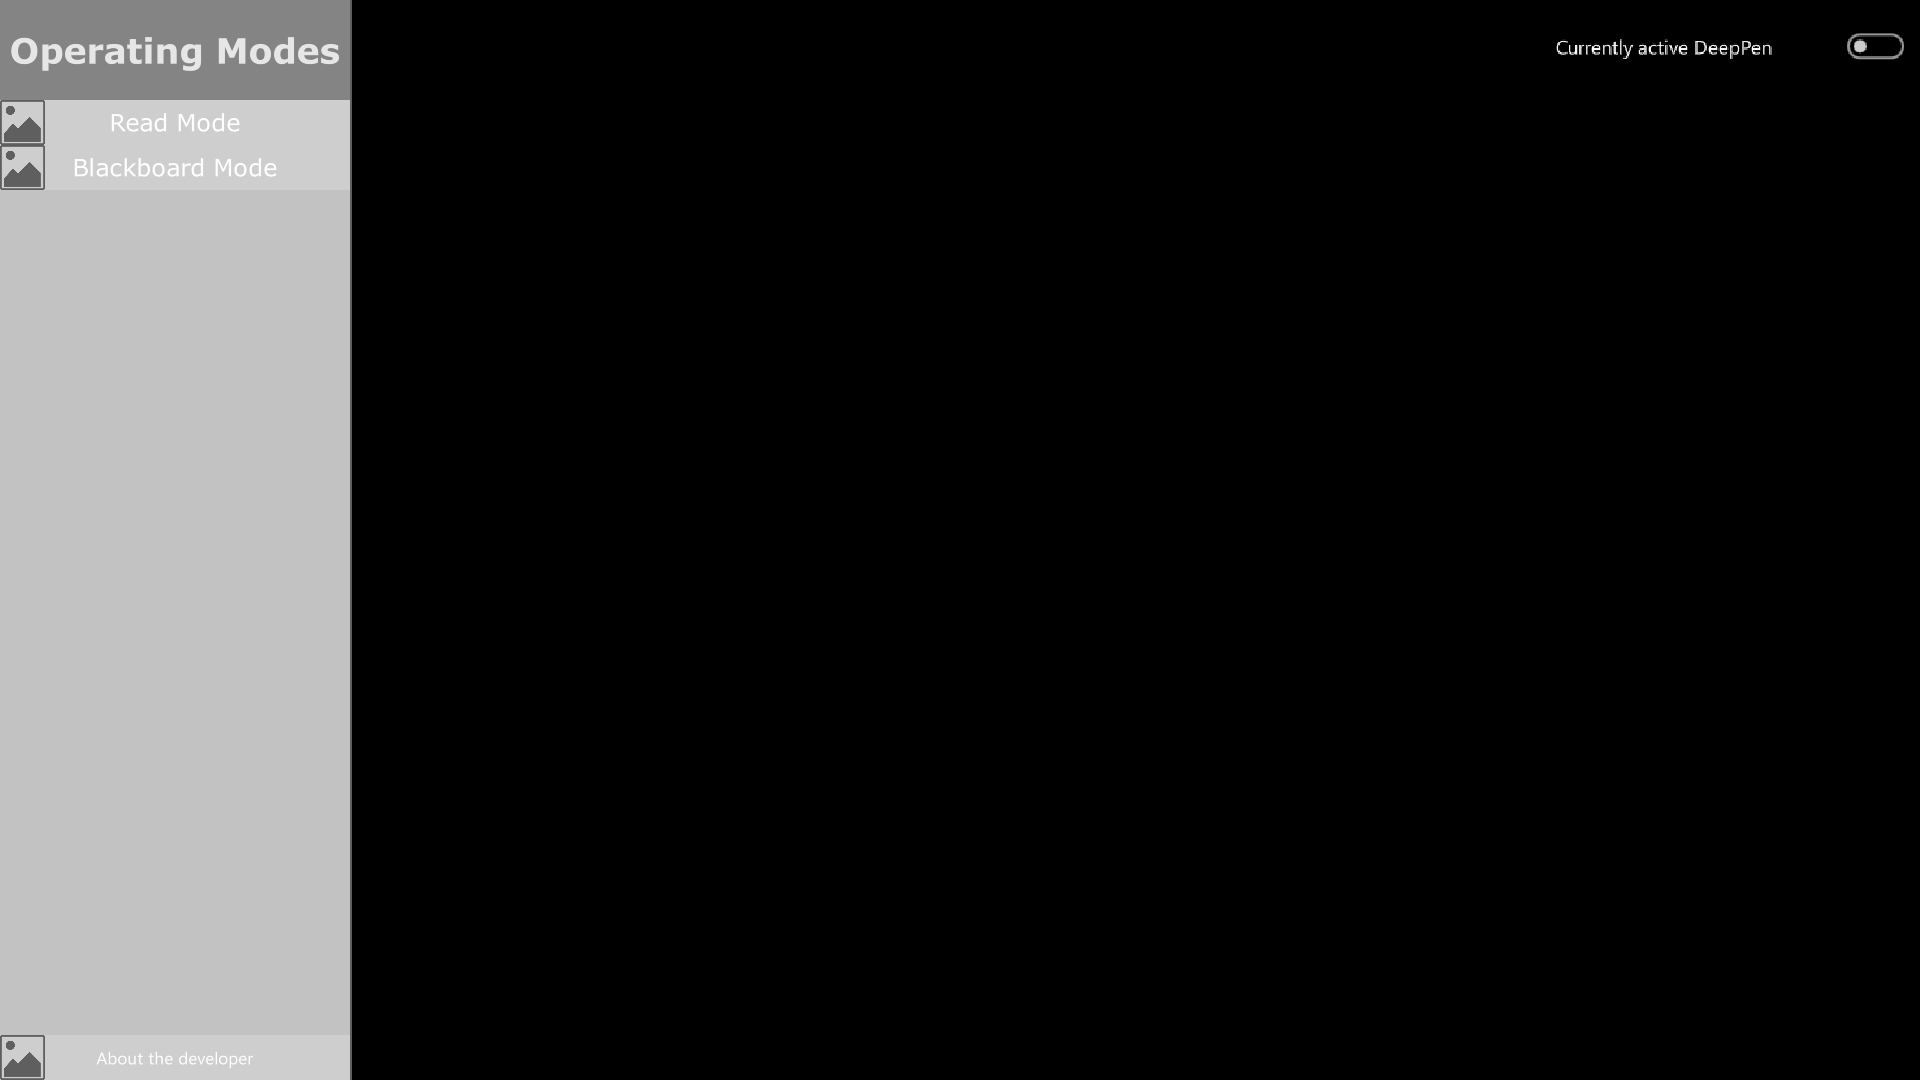
\includegraphics[width=1\textwidth]{capturas/DisenoUsuario1.png}\\[-0,40cm]
    \caption{Primer boceto en QT Design Studio}
    \end{figure}

Con este primer acercamiento, se dispusieron los elementos planteados como imprescindibles.
No obstante, al finalizar esta primera iteración de diseño, se evidenciaron
carencias a nivel estético; facilmente resolubles al comenzar con la
implementación real en \textbf{\textit{QT Creator}}. También se observó que faltaban
algunos botones como el de sincronización con el \textbf{\textit{DeepPen}},
que \textit{Read Mode} no era un buen nombre para indicar el comportamiento
del modo, o que había un espacio en el centro de la barra superior sin usar y
que podía usar para indicar el modo actual.\newline
Contando con estas consideraciones, pudieron corregirse en la siguiente iteración
de aproximación al diseño con el que partir en la implementación.

\begin{figure}[h]
    \centering
    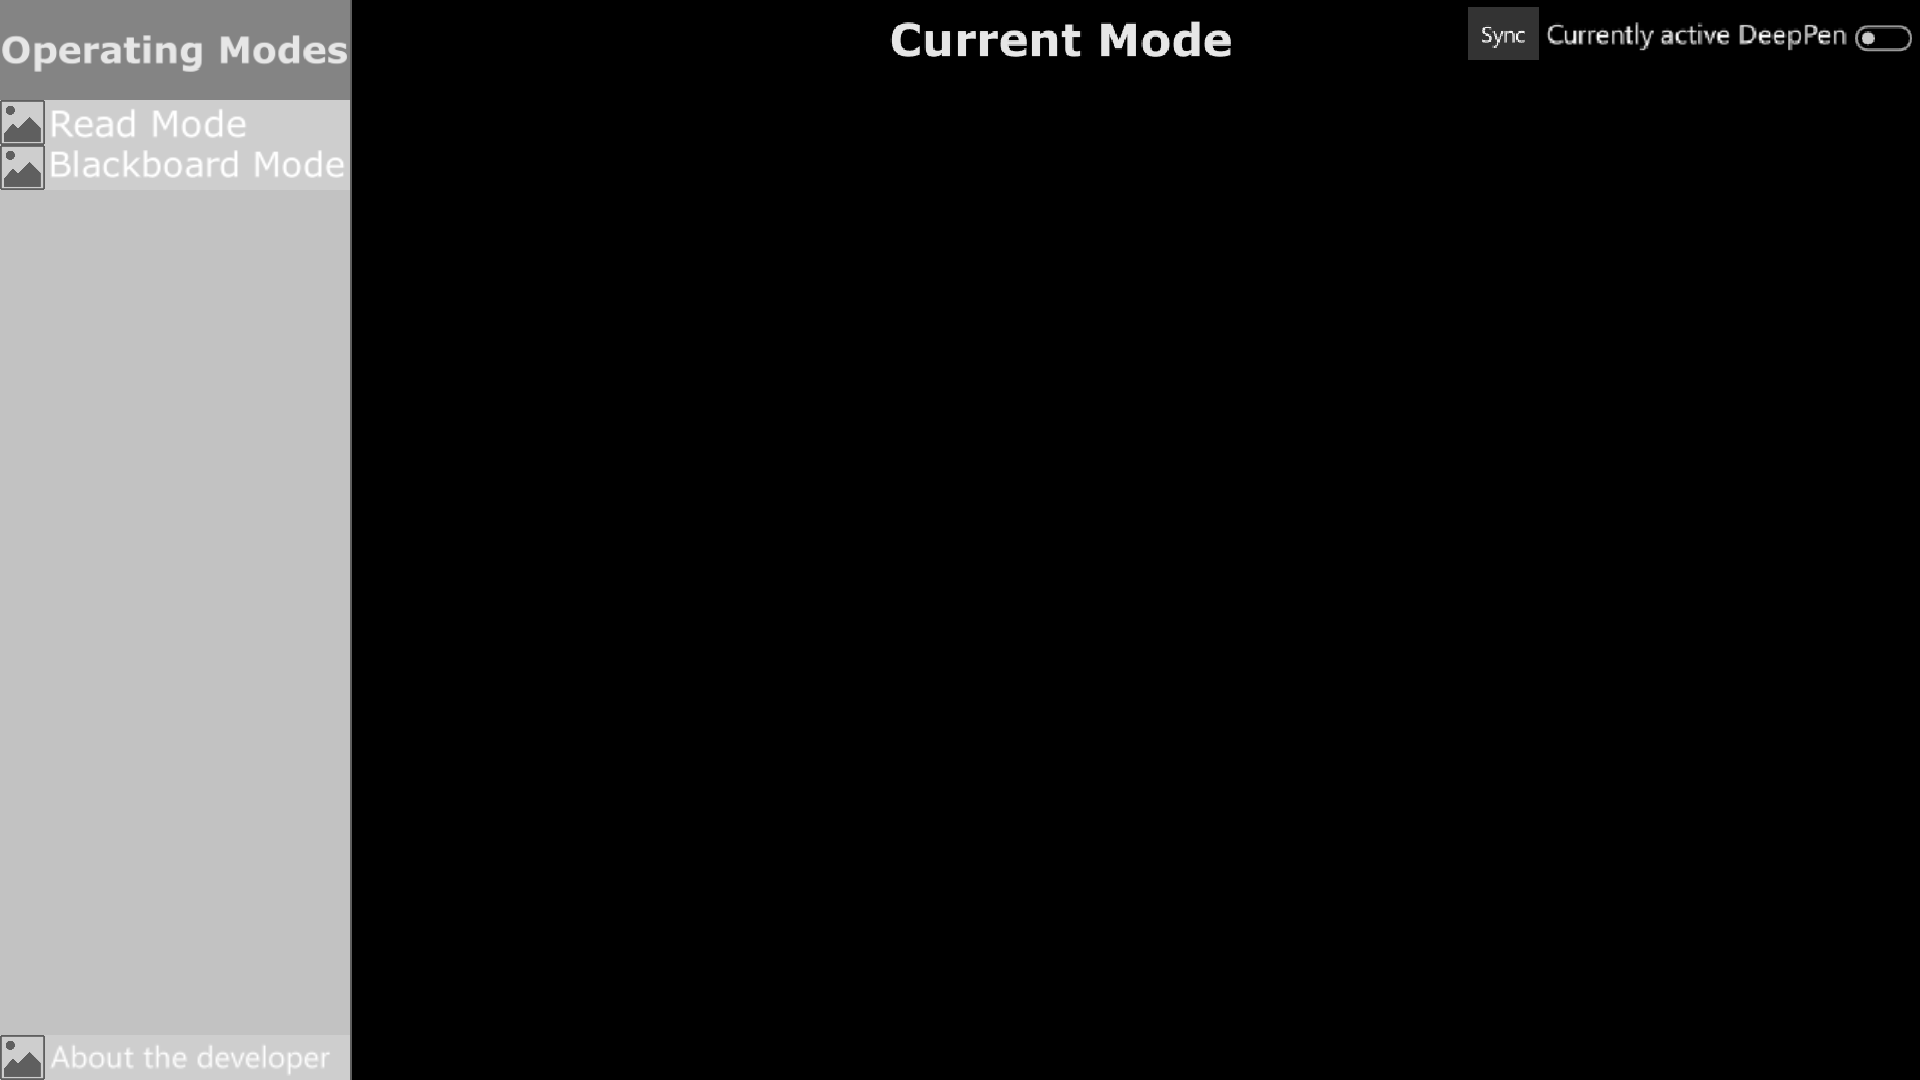
\includegraphics[width=1\textwidth]{capturas/DisenoUsuario2.png}\\[-0,40cm]
    \caption{Segundo boceto en QT Design Studio}
    \end{figure}

Para pasar esta aproximación de diseño a una implementación real, se utilizaron
\textbf{\textit{QT Creator}} con \textbf{\textit{C++}}. Resultando en lo siguiente:

\begin{figure}[h]
    \centering
    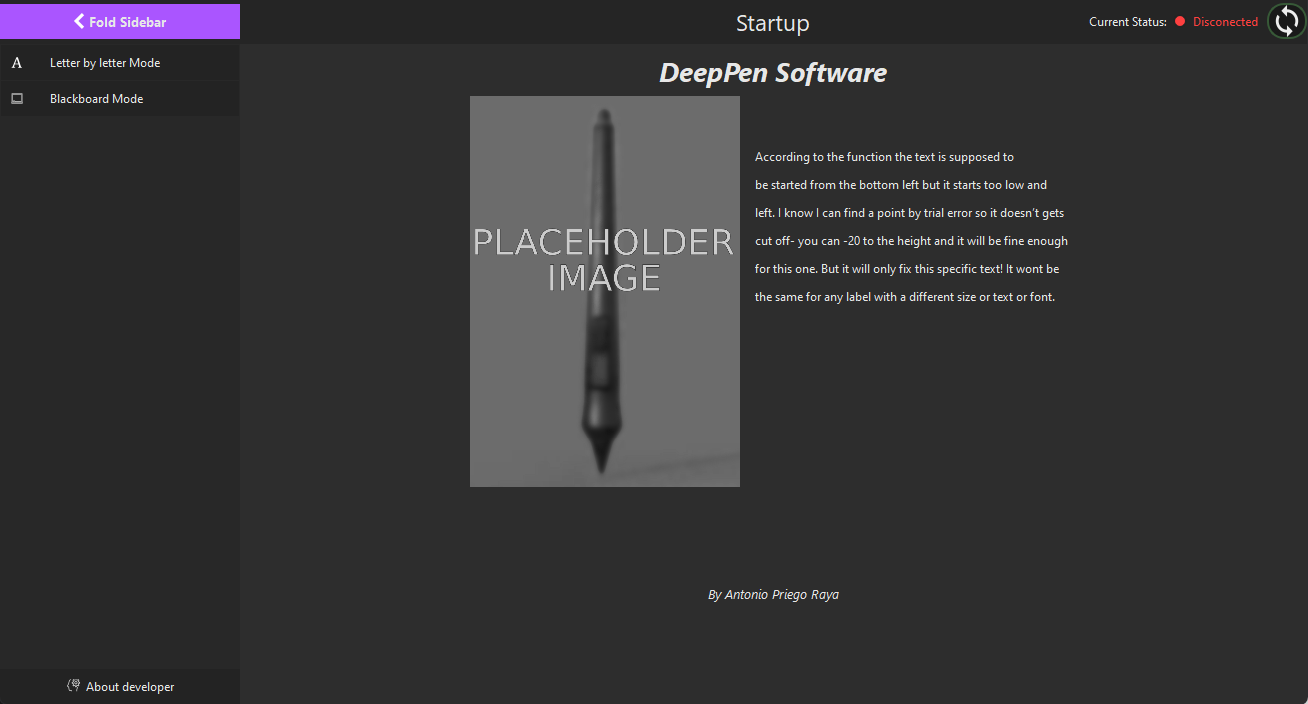
\includegraphics[width=1\textwidth]{capturas/Interfaz.png}\\[-0,40cm]
    \caption{Primera implementación de la interfaz de usuario del
    \textbf{\textit{DeepPen}}}
    \end{figure}

\section{Implementación}